\documentclass[a4paper,11pt]{book}
\usepackage[T1]{fontenc}
\usepackage[utf8]{inputenc}
\usepackage{lmodern}
\usepackage[banglamainfont=Kalpurush, 
            banglattfont=Siyam Rupali
           ]{latexbangla}
\usepackage[sexy,hints]{evan}
\usepackage{hyperref}
\usepackage{graphicx}
\usepackage[english]{babel}
\usetikzlibrary{decorations.markings}
\usepackage{amsmath}
\usepackage{dirtytalk}
\usepackage{mathtools}
\usepackage{tikz}
\usetikzlibrary{arrows,positioning} 
\usepackage{array}
\usepackage{wrapfig}
\usepackage{multirow}
\usepackage{tabu}
\usetikzlibrary{calc}
\usepackage{changepage}
\usepackage{caption,setspace}
\newcommand\perm[2][^n]{\prescript{#1\mkern-2.5mu}{}P_{#2}}
\newcommand\comb[2][^n]{\prescript{#1\mkern-0.5mu}{}C_{#2}}
\begin{document}

\chapter{Permutations and Combinations}

\section{Two Basic Counting Principles }
In our everyday lives, we often need to enumerate \say{events} such as, the 
arrangement of objects in a certain way, the partition of things under a 
certain condition, the distribution of items according to a certain specification, and so on. For instance, we may come across counting problems of 
the following types: 

\say{\textit{How many ways are there to arrange 5 boys and 3 girls in a row so 
that no two girls are adjacent?}}

\say{\textit{How many ways are there to divide a group of 10 people into three groups consisting of 4, 3 and 2 people respectively, with 1 person rejected? }}

These are two very simple examples of counting problems related to 
what we call \say{permutations} and \say{combinations}. Before we introduce in 
the next three sections what permutations and combinations are, we state 
in' this section two principles that are fundamental in all kinds of counting 
problems. \\

\begin{theorem}[The Addition Principle (AP) ]
Assume that there are:
\begin{center}
$n_{1}$ ways for the event  $E_{1}$ to occur,\\
$n_{2}$ ways for the event  $E_{2}$ to occur,\\
.\\
.\\
.\\
$n_{k}$ ways for the event  $E_{k}$ to occur,
\end{center}
where $k\ge 1$ If these ways for the different events to occur are pairwise disjoint, then the number of ways for at least one of the events 
$E_{1},E_{2},\cdots,$ or $E_{k}$ to occur is $n_{1}+ n_{2}+n_{3}+\cdots + n_{k} = \sum\limits_{i=1}^{k}  n_{i} $
\end{theorem}
\begin{example}
One can reach city $Q$ from city $P$ by sea, air and 
road. Suppose that there are 2 ways by sea, 3 ways by air and 2 ways by 
road (see Figure 1.1.1). Then by (AP), the total number of ways from $P$ 
to $Q$ by sea, air or road is 2 + 3 + 2 = 7. 
\end{example}
\begin{figure}[h]
\begin{center}
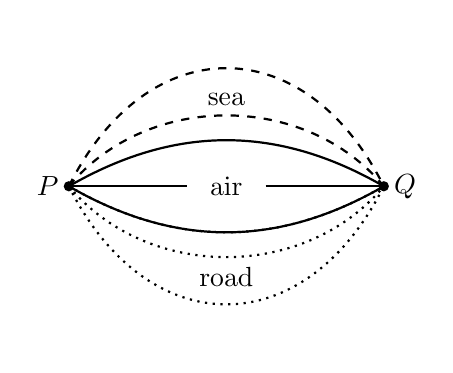
\begin{tikzpicture}[thick]
\def\upperarc{2}
\def\lowerarc{1.2}
\coordinate (P) at (0,0);
\coordinate (Q) at (4,0);
\foreach \x in {P,Q} {
  \draw[fill] (\x) circle (0.05);
}
\node[left] (P1) at (P) {$P$};
\node[right] (Q1) at (Q) {$Q$};
\coordinate (PQ) at ($(P)!.5!(Q)$);
\draw (P) -- ($(PQ)-(0.5,0)$);
\draw ($(PQ)+(0.5,0)$) -- (Q);
\node (air) at (PQ) {air};
\coordinate (CPQ1) at ($(PQ) - (1,0)$);
\coordinate (CPQ2) at ($(PQ) + (1,0)$);
\draw[dashed] let \p{1}=(CPQ1),\p{2}=(CPQ2) in (P) .. controls (\x1,\upperarc) and (\x2,\upperarc) .. (Q);
\draw[dashed] let \p{1}=(CPQ1),\p{2}=(CPQ2) in (P) .. controls (\x1,\lowerarc) and (\x2,\lowerarc) .. node[midway,above] {sea} (Q);
\draw (P) to [bend left=30]  (Q);
\draw (P) to [bend right=30]  (Q);
\draw[dotted] (P) to [bend right=30] (Q);
\draw[dotted] let \p{1}=(CPQ1),\p{2}=(CPQ2) in (P) .. controls (\x1,-\upperarc) and (\x2,-\upperarc) .. (Q);
\draw[dotted] let \p{1}=(CPQ1),\p{2}=(CPQ2) in (P) .. controls (\x1,-\lowerarc) and (\x2,-\lowerarc) .. node[midway,below] {road} (Q);
\end{tikzpicture}
\caption{•}
\end{center}
\end{figure}
An equivalent form of (AP), using set-theoretic terminology, is given 
below. 
\begin{lemma}
Let $A_{1}, A_{2}, A_{3}, \cdots , A_{k}$ be any $k$ finite sets, where $k \ge 1$. If the given sets are pairwise disjoint, i.e, $A_{i} \cap A_{j} = \phi$ for $i,j =1,2,\cdots, k, i\neq j$, then
\[ \abs{\bigcup_{i=0}^{k} A_{i}} = \abs{A_{1} \cup A_{2}\cup\cdots\cup A_{k}} = \sum_{i=0}^{k}\abs{A_{i}} \]
\end{lemma}
\begin{example}
Find the number of ordered pairs $(x, y)$ of integers such that $x^{2}+y^{2}\le 5.$ 
\end{example}
\begin{soln}
We may divide the problem into 6 disjoint cases: $x^{2}+y^{2} = 0,1,\cdots, 5$.Thus for $i= 0,1,\cdots, 5$, Let
\[ S_{i} = \{ (x,y)\,|\,x,y \in \ZZ, \, x^{2}+y^{2} =i \} \]
It can be checked that
\begin{flalign*} 
S_{0} &=  \{ (0,0) \}, \\ 
S_{1} &=  \{ (1, 0), (-1,0), (0,1), (0, -1)  \}, \\ 
S_{2} &=  \{(1, 1), (1, -1), (-1,1), (-1, -1)\},  \\ 
S_{3} &= \phi, \\
S_{4} &= \{(0, 2), (0, -2), (2, 0), (-2, 0)\}, and \\
S_{5} & = \{(1, 2), (1, -2), (2,1), (2, -1), (-1,2), (-1, -2), (-2,1), (-2, -1)\}. 
\end{flalign*}
Thus by (AP), the desired number of ordered pairs is 
\[ \sum_{i=0}^{5} \abs{S_{i}} = 1+4+4+0+4+8=21 \]
\end{soln}
\textbf{ Remark:}
  1) In the above example, one can find out the answer \say{21} simply by listing all the required ordered pairs $(x, y)$. The above method, 
however, provides us with a systematical way to obtain the answer.\\ 
2) One may also divide the above problem into disjoint cases: $x^2 = 
0,1,\cdots, 5$,  find out the number of required ordered pairs in each case, and 
obtain the desired answer by applying (AP). 
\begin{theorem}[The Multiplication Principle (MP) ]
Assume that an event E can be decomposed into r ordered events $E_{1},E_{2}, \cdots, E_{r}$ and that there are
\begin{center}
$n_{1}$ ways for the event  $E_{1}$ to occur,\\
$n_{2}$ ways for the event  $E_{2}$ to occur,\\
.\\
.\\
.\\
$n_{k}$ ways for the event  $E_{r}$ to occur,
\end{center}
Then the total number of ways for the event E to occur is given by: 
 \[n_{1}\times n_{2}\times n_{3} \times \cdots \times n_{r} = \prod_{i=1}^{r}  n_{i} \]
\end{theorem}

\begin{example}
To reach city $D$ from city $A$, one has to pass through city $B$ and then city $C$ as shown in Figure 1.1.2. If there are 2 ways to travel from $A$ to $B$, $5$ ways from $B$ to $C$, and $3$ ways from $C$ to $D$, then by (MP), the number of ways from $A$ to $D$ via $B$ and $C$ is given by $2 \times 5 \times 3 = 30.$ 
\end{example}
\begin{figure}[h]
\begin{center}
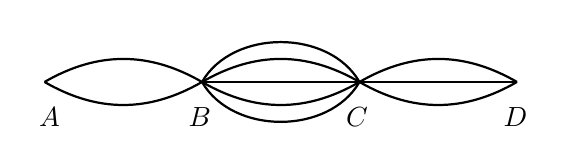
\begin{tikzpicture}[thick]
\def\upperarc{2}
\def\lowerarc{1.2}
\coordinate (A) at (0,0);
\coordinate (B) at (2,0);
\coordinate (C) at (4,0);
\coordinate (D) at (6,0);
\draw (-.2,-.2) node[anchor=north west] {$A$};
\draw (1.7,-.2) node[anchor=north west] {$B$};
\draw (3.7,-.2) node[anchor=north west] {$C$};
\draw (5.7, -.2) node[anchor=north west] {$D$};
\draw (A) to [bend left=30]  (B);
\draw (A) to [bend right=30]  (B);
\draw (B) to (C);
\draw (B) to [bend left=30]  (C);
\draw (B) to [bend left= 60]  (C);
\draw (B) to [bend right=30]  (C);
\draw (B) to [bend right=60]  (C);
\draw (C) to [bend left=30]  (D);
\draw (C) to [bend right=30]  (D);
\draw (C) to (D);
\end{tikzpicture}
\caption{}
\end{center}
\end{figure}

An equivalent form of (MP) using set-theoretic terminology, is stated 
below. 
\begin{lemma}
Let,
\[ \prod_{i=1}^{r} A_{i} = A_{1} \times A_{2} \times A_{3} \cdots \times A_{r} = \{ (a_{1}, a_{2}, a_{3}, \cdots , a_{r}) |a_{i} \in A_{i},\; i = 1,2,3,\cdots, r\}       \]
 denote the cartesian product of the finite sets $A_{1}, A_{2}, A_{i},\cdots, A_{r}$. Then
 \[ \abs{\prod_{i=0}^{r} A_{i}} = \abs{A_{1}} \times \abs{A_{2}} \times \cdots \times \abs{A_{r}} = \prod_{i=1}^{r}\abs{A_{i}} \]
\end{lemma}
A sequence of numbers $a_{1},a_{2},a_{3},\cdots,a_{n}$ is called a $k-ary\, sequence$, where $n, k \in \NN,$ if $a_{i} \in \{0, 1, \cdots, k - 1\}$ for each $i = 1, 2, \cdots, n.$ The length of the sequence  $a_{1},a_{2},a_{3},\cdots,a_{n}$ is defined to be $n$, which is the number of terms contained in the sequence. At times, such a sequence may be denoted by $(a_{1},a_{2},a_{3},\cdots,a_{n})$ A $k-ary\, sequence$ is also called a $binary$, $ternary$, or $quaternary$ sequence when $k = 2, 3\, or\, 4$, respectively. Thus, $\{000, 001,010,100,011,101,110, 111\}$ is the set of all $8(= 2^3)$ binary sequences of length 3. For given $k, n \in \NN$, how many different $k-ary\, sequences$ of length $n$ can we form? This will be discussed in the following example. You will find the result useful later on. 
\begin{example}
To form a $k-ary\, sequence \quad a_{1},a_{2},a_{3},\cdots,a_{n}$ of length $n$, we first select an $a_1$ from the set $B = \{0, 1, ..., k - 1\};$ then an $a_2$ from the same set $B;$ and so on until finally an $a_n$ again from $B$. Since there are $k$ choices in each step, the number of distinct $k-ary\, sequences$ of length $n$ is, by (MP), $\underbrace{k\times k \times k \times \cdots \times k}_{n} = k^{n}$
\end{example}
\begin{example}
Find the number of positive divisors of 600, inclusive of 1 and 600 itself. 
\end{example}
\begin{soln}
We first note that the number $'600'$ has a unique prime factorization, namely, $600 = 2^3 \times 3^1 \times 5^2.$ It thus follows that a positive 
integer $m$ is a divisor of $600$ if and only if $m$ is of the form $m = 2^{a} \times 3^{b}\times 5^{c} $, where $a, b, c \in \ZZ$ such that $0 < a < 3$, $0 < b < 1$ and $0 < c < 2$. Accordingly, the number of positive divisors of $'600'$ is the number of ways to form the 
triples $(a, b, c)$ where $a \in \{0, 1,2, 3\}, b \in \{0, 1\}$ and $c \in \{0, 1, 2\}$, which by (MP), is equal to $4 \times 2 \times 3 = 24.$ 
\end{soln}

\textbf{ Remark:}
By applying (MP) in a similar way, one obtains the following 
general result. \\
\textit{If a natural number $n$ has as its prime factorization, }
\[ n = p_{1}^{k_{1}}\times p_{2}^{k_{2}} \times \cdots \times p_{r}^{k_{r}}   \]
\textit{where the $p_{i}$'s are distinct primes and the $k_i$ 's are positive integers, then the number of positive divisors of $n$ is given by $\prod\limits_{i=1}^{r}(k_{i}+1)$. }\\
In the above examples, we have seen how (AP) and (MP) were separately used to solve some counting problems. Very often, solving a more 
complicated problem may require a 'joint' application of both (AP) and 
(MP). To illustrate this, we give the following example. 
\begin{example}
Let $X = \{1,2,3\cdots 100 \}$ and let
\[ S = \{(a,b,c)| a,b,c\in X, a<b\, \text{and}\, a<c \} \]
Find $|S|$.
\end{example}

\begin{soln}
The problem may be divided into disjoint cases by considering $a = 1, 2,\cdots, 99.$ For $a = k\in \{1, 2, \cdots, 99\},$ the number of choices for $b$ is $100 - k$ and that for $c$ is also $100 - k$. Thus the number of required ordered triples $(k, b, c)$ is $(100 - k)^2$, by (MP). Since k takes on the values $1,2, \cdots,99$ by applying (AP), we have 
\[\abs{S} = 99^2 + 98^2 +\cdots + 1^2 .\] 
Using the formula $\sum\limits_{k=1}^{n} k^2 = \dfrac{n(n + 1)(2n + 1)}{6} $, we finally obtain 

\[ \abs{S} = \frac{1}{6} \times 99 \times 100 \times199 = 328350. \] 
\end{soln}
As mathematical statements, both (AP) and (MP) are really 'trivial'. 
This could be a reason why they are very often neglected by students. Actually, they are very fundamental in solving counting problems. As we shall witness in this book, a given counting problem, no matter how complicated it is, can always be 'decomposed' into some simpler 'sub-problems' that in turn can be counted by using (AP) and/or (MP). \\

\section{Permutations}
At the beginning of Section 1.1, we mentioned the following problem: "How many ways are there to arrange 5 boys and 3 girls in a row so that no two girls are adjacent?" This is a typical example of a more general problem of arranging some distinct objects subject to certain additional conditions. \\

Let $A = \{a_1, a_2,\cdots, a_n\}$ be a given set of $n$ distinct objects. For $0 \le r \le n$, an $r-$permutation of $A$ is a way of arranging any $r$ of the objects of $A$ in a row. When $r = n$, an $n-$permutation of $A$ is simply called a permutation of $A$. 
\begin{example}
Let $A = \{a, b, c, d\}$. All the 3-permutations of A are shown below: 
\begin{align*}
& abc, acb, bac, bca, cab, cba\\
& abd, adb, bad, bda, dab, dba \\
& acd, adc, cad, cda,  dac, dca \\ 
& bcd, bdc, cbd, cdb, dbc, dcb
\end{align*}

There are altogether 24 in number. . 
\end{example}
Let $\perm[n]{r}$ denote the number of $r-permutations$ of $A$. Thus $\perm[3]{4} = 24$ as shown in Example 1.2.1. In what follows, we shall derive a formula for $\perm[r]{n}$  by applying (MP). \\

An $r-permutation$ of $A$ can be formed in $r$ steps, as described below: 
First, we choose an object from $A$ and put it in the first position (see 
Figure 1.2.1). Next we choose an object from the remaining ones in $A$ and 
put it in the second position. We proceed on until the $r-{th}$ step in which we choose an object from the remaining $(n - r + 1)$ elements in $A$ and put it in the $r-{th}$ position. \\

\begin{figure}[h]
\begin{center}
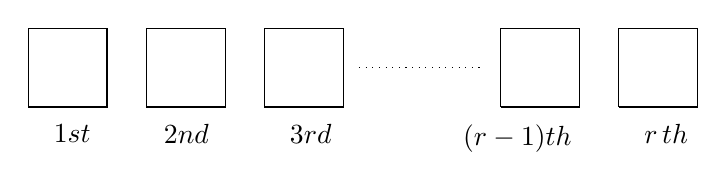
\begin{tikzpicture}
\draw (0,0) -- (1,0) -- (1,1) -- (0,1) -- (0,0);
\draw (1.5,0) -- (2.5,0) -- (2.5,1) -- (1.5,1) -- (1.5,0);
\draw (3,0) -- (4,0) -- (4,1) -- (3,1) -- (3,0);
\draw [dotted] (4.2,.5) -- (5.8,.5);
\draw (6,0) -- (7,0) -- (7,1) -- (6,1) -- (6,0);
\draw (7.5,0) -- (8.5,0) -- (8.5,1) -- (7.5,1) -- (7.5,0);
\draw (.2,-.1) node[anchor=north west] {$1st$};
\draw (1.6,-.1) node[anchor=north west] {$2nd$};
\draw (3.2,-.1) node[anchor=north west] {$3rd$};
\draw (5.4,-.1) node[anchor=north west] {$(r-1)th$};
\draw (7.7,-.1) node[anchor=north west] {$r\,th$};
\end{tikzpicture}
\end{center}
\caption{•}
\end{figure}



There are $n$ choices in step $1, (n - 1)$ choices in step $2,\cdots, n - (r - 1)$ 
choices in step $r$. Thus by (MP), 
\[ \perm[n]{r} = n(n - 1)(n - 2)\cdots (n - r + 1).\] 

If we use the factorial notation: $n! = n \times (n - 1) \times \cdots \times 2 \times 1$, then 

\[ \perm[n]{r} = \dfrac{n!}{(n-r)!}\]

\textbf{ \textit{ Remark}}. By convention, $O! = 1$. Note that $\perm[n]{0} = 1$ and  $\perm[n]{n} = n!$. 
\begin{example}
Let $E = \{a,b,c,\cdots,x,y,z\}$ be the set of the 26 English alphabets. Find the number of 5-letter words that can be formed from $E$ such that the first and last letters are distinct vowels and the remaining three are distinct consonants. 
\end{example}

\begin{figure}[h]
\begin{center}
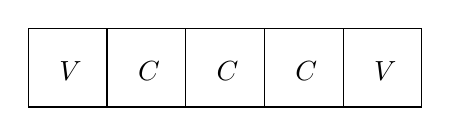
\begin{tikzpicture}
\draw (0,0) -- (5,0) -- (5,1) -- (0,1) -- (0,0);
\draw (1,0) -- (1,1);
\draw (2,0) -- (2,1);
\draw (3,0) -- (3,1);
\draw (4,0) -- (4,1);
\draw (.27,.7) node[anchor=north west] {$V$};
\draw (4.27,.7) node[anchor=north west] {$V$};
\draw (1.27,.7) node[anchor=north west] {$C$};
\draw (2.27,.7) node[anchor=north west] {$C$};
\draw (3.27,.7) node[anchor=north west] {$C$};
\end{tikzpicture}
\caption{•}
\end{center}
\end{figure}

\begin{soln}
There are 5 vowels and 21 consonants in $E$. A required 5-letter word can be formed in the following way. \\
\textbf{ \textit{ Step 1.}} Choose a 2-permutation of $\{a, e, i, o, u\}$ and then put the first vowel in the $1^{st}$ position and the second vowel in the $5^{th}$ position (see Figure 1.4). \\
\textbf{\textit{ Step 2.}} Choose a 3-permutation of $E\setminus \{a, e, i, o, u\}$ and put the $1st$, $2nd$ and $3rd$ consonants of the permutation in the $2nd$, $3rd$ and $4th$ positions respectively (see Figure 1.4). \\

There are $\perm[5]{2}$ choices in Step 1 and $\perm[21]{3}$ choices in Step 2. Thus by (MP), the number of such 5-1etter words is given by 
\[\perm[5]{2}\times \perm[21]{3} = (5 \times 4) \times (21 \times 20 \times 19) = 159600. \]
\end{soln}

\begin{example}
There are 7 boys and 3 girls in a gathering. In how many ways can they be arranged in a row so that \\
$(i)$ the 3 girls form a single block (i.e. there is no boy between any two of 
the girls)? \\
$(ii)$ the two end-positions are occupied by boys and no girls are adjacent? 
\end{example}

\begin{soln}
$(i)$ Since the 3 girls must be together, we can treat them as a single entity. The number of ways to arrange 7 boys together with this entity is $(7 + 1)!$. As the girls can permute among themselves within the entity in $3!$ ways, the desired number of ways is, by (MP), 
\[8! \times 3!\] 
$(ii)$ We first consider the arrangements of boys and then those of girls. 
There are $7!$ ways to arrange the boys. Fix an arbitrary one of the arrangements. Since the end-positions are occupied by boys, there are only 6 spaces available for the 3 girls $G_1$, $G_2$ and $G_3$ . \\
\begin{figure}[h]
\begin{center}
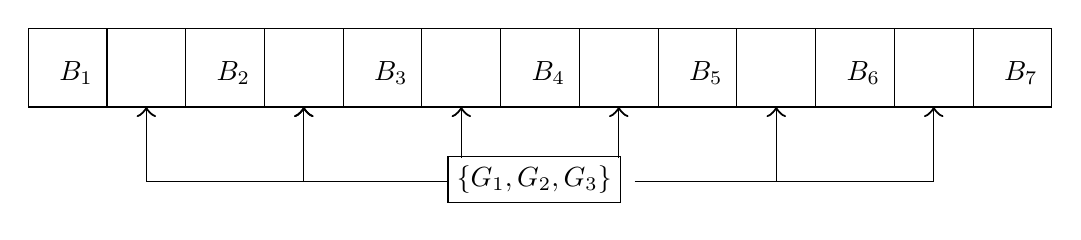
\begin{tikzpicture}
\draw (0,0) -- (13,0) -- (13,1) -- (0,1) -- (0,0);
\draw (1,0) -- (1,1);
\draw (2,0) -- (2,1);
\draw (3,0) -- (3,1);
\draw (4,0) -- (4,1);
\draw (5,0) -- (5,1);
\draw (6,0) -- (6,1);
\draw (7,0) -- (7,1);
\draw (8,0) -- (8,1);
\draw (9,0) -- (9,1);
\draw (10,0) -- (10,1);
\draw (11,0) -- (11,1);
\draw (12,0) -- (12,1);
\draw (5.32,-.95) -- (1.5,-.95);
\draw (7.7,-.95) -- (11.5,-.95);
\draw [  decoration={markings,mark=at position 1 with {\arrow[scale=2]{>}}},
    postaction={decorate},
    shorten >=0.4pt] (1.5,-.95)--(1.5,0);
\draw [  decoration={markings,mark=at position 1 with {\arrow[scale=2]{>}}},
    postaction={decorate},
    shorten >=0.4pt] (3.5,-.95)--(3.5,0);
\draw [  decoration={markings,mark=at position 1 with {\arrow[scale=2]{>}}},
    postaction={decorate},
    shorten >=0.4pt] (3.5,-.95)--(3.5,0);
\draw [  decoration={markings,mark=at position 1 with {\arrow[scale=2]{>}}},
    postaction={decorate},
    shorten >=0.4pt] (5.5,-.65)--(5.5,0);
\draw [  decoration={markings,mark=at position 1 with {\arrow[scale=2]{>}}},
    postaction={decorate},
    shorten >=0.4pt] (7.5,-.65)--(7.5,0);
\draw [  decoration={markings,mark=at position 1 with {\arrow[scale=2]{>}}},
    postaction={decorate},
    shorten >=0.4pt] (9.5,-.95)--(9.5,0);
\draw [  decoration={markings,mark=at position 1 with {\arrow[scale=2]{>}}},
    postaction={decorate},
    shorten >=0.4pt] (11.5,-.95)--(11.5,0);
\draw (.27,.7) node[anchor=north west] {$B_1$};
\draw (2.27,.7) node[anchor=north west] {$B_2$};
\draw (4.27,.7) node[anchor=north west] {$B_3$};
\draw (6.27,.7) node[anchor=north west] {$B_4$};
\draw (8.27,.7) node[anchor=north west] {$B_5$};
\draw (10.27,.7) node[anchor=north west] {$B_6$};
\draw (12.27,.7) node[anchor=north west] {$B_7$};
\draw (5.2,-.5) node[anchor=north west] {$\boxed{\{G_1, G_2, G_3\} }$};
\end{tikzpicture}
\caption{•}
\end{center}
\end{figure}

$G_1$ has 6 choices. Since no two girls are adjacent, $G_2$ has 5 choices and $G_3$ has 4. Thus by (MP), the number of such arrangements is 
\[7! \times 6 \times 5 \times 4. \] 
\end{soln}
\textbf{Remark} Example 1.2.3 can also be solved by considering the arrangements for the girls first. This will be discussed in Example 1.7.2. 
\begin{example}
Between 20000 and 70000, find the number of even integers in which no digit is repeated. 
\end{example}
\begin{soln}
Let $abcde$ be a required even integer. As shown in the following diagram, the 1st digit a can be chosen from $\{2, 3,4,5, 6\}$ and the 5th digit e can be chosen from $\{0, 2,4,6, 8\}$. 
Since $\{2, 3,4,5, 6\} \cap \{0, 2,4,6, 8\} = \{2, 4, 6\}$, we divide the problem into 2 disjoint cases: \\

\textbf{\textit{ Case 1}}. $a \in \{2, 4, 6\}$. In this case, $a$ has 3 choices, $e$ then has $4(= 5 - 1)$ choices, and $bed$ has $\perm[(10-2)]{3} = \perm[8]{3}$ choices. By (MP), there are 
\[3 \times 4 \times  \perm[8]{3} = 4032 \]
such even numbers. \\

\textbf{\textit{ Case 2.}} $a \in \{3, 5\}$. In this case, $a$ has 2 choices, $e$ has 5 choices and again $bed$ has $\perm[8]{3}$ choices. By (MP), there are 
\[2 \times 5 \times  \perm[8]{3} = 3360\] 
such even numbers\\. 
Now, by (AP), the total number of required even numbers is $4032 + 
3360 = 7392. $
\end{soln}

\begin{example}
Let $S$ be the set of natural numbers whose digits are chosen from $\{1, 3, 5, 7\}$ such that no digits are repeated. Find \\
\[(i)\, \abs{S} \quad (ii)\, \sum\limits_{n\in S} n\]
\end{example}

\begin{soln}
$(i)$ We divide S into 4 disjoint subsets consisting of:\\ 
$(1)\,1-$ digit numbers: $1,3,5,7;$ \\
$(2)\, 2-$ digit numbers: $13, 15, \cdots;$ \\
$(3)\, 3-$ digit numbers: $135, 137, \cdots;$ \\
$(4)\, 4-$ digit numbers: $1357, 1375, \cdots;$ \\
and find $|S|$ by applying (AP). Thus for $i = 1,2,3,4,$ let $S_{i}$ denote the 
set of $i-$digit natural numbers formed by $1,3,5,7$ with no repetition. Then 
$S = S_1 \cup S_2 \cup S_3 \cup S_4$ and by (AP), 
\begin{align*}
 |S| = \sum\limits_{i=1}^{4} |S_{i}| &= \perm[4]{1} + \perm[4]{2} + \perm[4]{3} + \perm[4]{4} \\
     &= 4+12+24+24 
 \end{align*}
$(ii)$ Let $\alpha = \sum\limits_{n\in S} n $. It is tedious to determine $\alpha$ by summing up all the 64 numbers in $S$. Instead, we use the following method. \\

Let $\alpha_{1}$ denote the sum of unit-digits of the numbers in $S;\,\alpha_{2}$ that of ten-digits of the numbers in $S;\,\alpha_{3}$ that of hundred-digits of the numbers in $S$; and $\alpha_4$ that of thousand-digits of the numbers in $S$. Then 
\[ \alpha = \alpha_{1} + 10\alpha_{2} + 100\alpha_{3} + 1000\alpha_{4}  \]
We first count $\alpha_{1}$. Clearly, the sum of unit-digits of the numbers in $S_{1}$ is
\[1 + 3 + 5 + 7 = 16. \]
In $S_2$, there are $\perm[3]{1}$ numbers whose unit-digits are, respectively, 1, 3, 5 and 7. Thus the sum of the unit-digits of the number is $S_2$ is 
\[ \perm[3]{1} \times (1 + 3 + 5 + 7) = 3 \times 16 = 48.\] 
In $S3$, there are $\perm[3]{2}$ numbers whose unit-digits are, respectively, 1, 3, 5 and 7. Thus the sum of unit-digits of the numbers in $S_3$ is 
\[ \perm[3]{2} \times (1 + 3 + 5 + 7) = 6 \times 16 = 96. \]
In $S_4$, there are $\perm[3]{3}$ numbers whose unit-digits are, respectively, 1, 3, 5 and 
7. Thus the sum of unit-digits of the numbers in $S_4$ is 
\[ \perm[3]{3} \times (1 + 3 + 5 + 7) = 6 \times 16 = 96. \]
Hence by (AP), 
\[ \alpha_{1} = 16 + 48 + 96 + 96 = 256. \]
Similarly, we have: 
\begin{align*}
 \alpha_2 &= \perm[3]{1} \times (1 + 3 + 5 + 7) + \perm[3]{2} \times (1 + 3 + 5 + 7) + \perm[3]{3} \times (1 + 3 + 5 + 7) = 240; \\
\alpha_{3} &=(\perm[3]{2} + \perm[3]{3}) \times (1 + 3 + 5 + 7) = 192;\\ 
 and\quad \alpha_{4} &=\perm[3]{3} \times (1 + 3 + 5 + 7) = 96. 
\end{align*} 
Thus, 
\begin{align*}
 \alpha &= \alpha_{1} + 10\alpha_{2} + 100\alpha_{3} + 1000\alpha_{4}  \\
 &=  256 + 2400 + 19200 + 96000\\ 
 &= 117856. 
\end{align*}
\end{soln}
\textbf{Remark:} There is a shortcut to compute the sum $\alpha = \sum( n | n \in S)$ in part $(ii)$. Observe that the 4 numbers in $S_{1}$ can be paired off as $\{1, 7\}$ and $\{3,5\}$ so that the sum of the two numbers in each pair is equal to 8 and the 12 numbers in $S_2$ can be paired off as $\{13,75\}$, $\{15,73\}$, $\{17, 71\}$, $\{35, 53\}, \cdots $so that the sum of the two numbers in each pair is 88. Likewise, the 24 numbers in $S_3$ and the 24 numbers in $S_4$ can be paired off so that the sum of the two numbers in each pair is equal to 888 and 8888 respectively. Thus 
\begin{align*}
\alpha &= 8 \times \frac{4}{2} + 88 \times \frac{12}{2} + 888 \times \frac{24}{2} + 8888\times \frac{24}{2}\\ 
&= 117856. 
\end{align*}
\section{Circular Permutation}
The permutations discussed in Section 1.2 involved arrangements of objects 
in a row. There are permutations which require arranging objects in a 
circular closed curve. These are called circular permutations. 
Consider the problem of arranging 3 distinct objects a, b, c in 3 positions 
around a circle. Suppose the 3 positions are numbered (1), (2) and (3) as 
shown in Figure 1.6 Then the three arrangements of $a,\; b,\; c$ shown in the 
figure can be viewed as the permutations:
\[ abc,\, cab,\, bca \] 
respectively. 

\begin{figure}[h]
\begin{center}
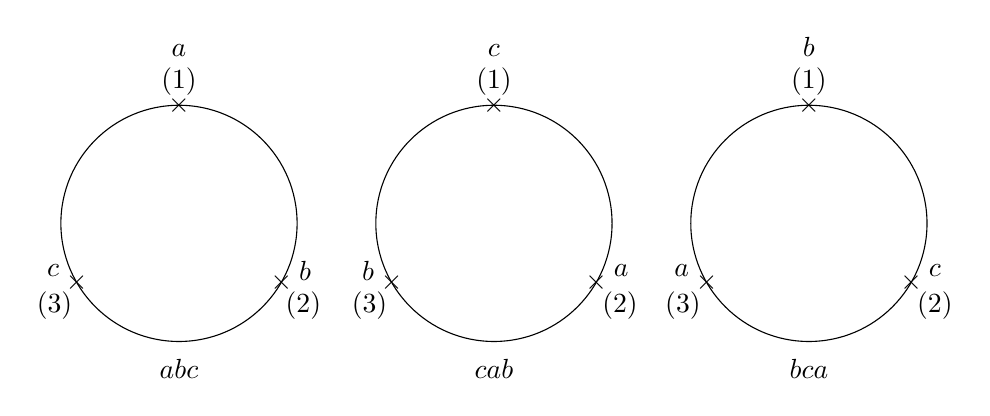
\begin{tikzpicture}
\draw (0,0) circle (1.5cm);
\draw (-4,0) circle (1.5cm);
\draw (4,0) circle (1.5cm);
\coordinate[label=above :(1)] (B) at (0,1.5);
\coordinate[label=above :(1)] (A) at (-4,1.5);
\coordinate[label=above :(1)] (F) at (4,1.5);
\coordinate[label=above :$c$] (C) at (0,2);
\coordinate[label=above :$a$] (D) at (-4,2);
\coordinate[label=above :$b$] (E) at (4,2);
\draw (0,1.5) node {$\times$};
\draw (4,1.5) node {$\times$};
\draw (-4,1.5) node {$\times$};
\draw (-1.29903810568,-.75) node {$\times$};
\draw (-5.29903810568,-.75) node {$\times$};
\draw (2.70096189432,-.75) node {$\times$};
\draw (1.29903810568,-.75) node {$\times$};
\draw (-2.70096189432,-.75) node {$\times$};
\draw (5.29903810568,-.75) node {$\times$};
\coordinate[label=left :$b$] (C) at (-1.40,-.60);
\coordinate[label=right :$a$] (C) at (1.40,-.60);
\coordinate[label=left :$c$] (C) at (-5.40,-.60);
\coordinate[label=right :$b$] (C) at (-2.60,-.60);
\coordinate[label=left :$a$] (C) at (2.6,-.60);
\coordinate[label=right :$c$] (C) at (5.40,-.60);
\coordinate[label=below :(3)] (C) at (-1.58,-.75);
\coordinate[label=below :(3)] (C) at (-5.58,-.75);
\coordinate[label=below :(3)] (C) at (2.40,-.75);
\coordinate[label=below :(2)] (C) at (-2.42,-.75);
\coordinate[label=below :(2)] (C) at (1.6,-.75);
\coordinate[label=below :(2)] (C) at (5.6,-.75);
\coordinate[label=below :$abc$] (C) at (-4,-1.6);
\coordinate[label=below :$cab$] (C) at (0,-1.6);
\coordinate[label=below :$bca$] (C) at (4,-1.6);
\end{tikzpicture}
\caption{•}
\end{center}
\end{figure}

In this case, such "$circular\, permutations$" are identical with the usual 
permutations, and thus there is nothing new worth discussing. To get 
something interesting, let us now neglect the numbering of the positions 
(and thus only "relative positions" of objects are concerned). As shown in 
Figure 1.3.2, any of the 3 arrangements is a rotation of every other; i.e., the 
relative positions of the objects are invariant under rotation. In this case, 
we shall agree to say that the 3 arrangements of Figure 1.3.2 are identical. 
In general, two circular permutations of the same objects are identical if 
anyone of them can be obtained by a rotation of the other. 
\begin{figure}[h]
\begin{center}
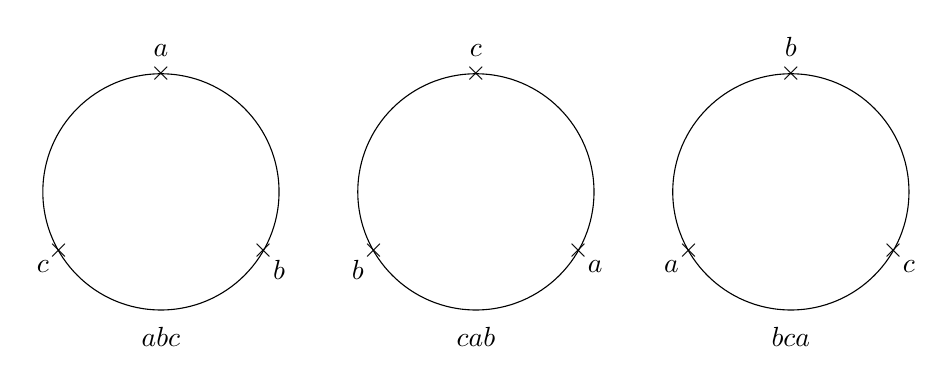
\begin{tikzpicture}
\draw (0,0) circle (1.5cm);
\draw (-4,0) circle (1.5cm);
\draw (4,0) circle (1.5cm);
\coordinate[label=above :$c$] (C) at (0,1.6);
\coordinate[label=above :$a$] (D) at (-4,1.6);
\coordinate[label=above :$b$] (E) at (4,1.6);
\draw (0,1.5) node {$\times$};
\draw (4,1.5) node {$\times$};
\draw (-4,1.5) node {$\times$};
\draw (-1.29903810568,-.75) node {$\times$};
\draw (-5.29903810568,-.75) node {$\times$};
\draw (2.70096189432,-.75) node {$\times$};
\draw (1.29903810568,-.75) node {$\times$};
\draw (-2.70096189432,-.75) node {$\times$};
\draw (5.29903810568,-.75) node {$\times$};
\coordinate[label=below left :$b$] (C) at (-1.29903810568,-.75);
\coordinate[label=below right :$a$] (C) at (1.29903810568,-.75);
\coordinate[label=below left :$c$] (C) at (-5.29903810568,-.75);
\coordinate[label=below right :$b$] (C) at (-2.70096189432,-.75);
\coordinate[label=below left :$a$] (C) at (2.70096189432,-.75);
\coordinate[label=below right :$c$] (C) at (5.29903810568,-.75);
\coordinate[label=below :$abc$] (C) at (-4,-1.6);
\coordinate[label=below :$cab$] (C) at (0,-1.6);
\coordinate[label=below :$bca$] (C) at (4,-1.6);
\end{tikzpicture}
\caption{•}
\end{center}
\end{figure}

Let $A$ be a set of n distinct objects. For $0 < r < n$, an $r-circular\, 
permutation$ of $A$ is a circular permutation of any $r$ distinct objects taken from $A$. Let $Q_{n}^{r}$ denote the number of $r-circular\, permutations$ of $A$. We shall derive a formula for  $Q_{n}^{r}$.\\

Let $A = \{a,b,c,d\}$. There are altogether $\perm[4]{3}(= 24)$ 
3-permutations of A and they are shown in Example 1.2.1. These 24 3-permutations are re-grouped into 8 subsets as shown below: 
\begin{center}
\begin{tabular}{ |c|c| } 
 \hline
 $abc\quad cab\quad  bca$ &  $acb\quad  bac\quad  cba$\\
\hline   
 $abd\quad  dab\quad  bda$ &  $adb\quad  bad\quad  dba$\\ 
 \hline
$acd\quad  dac\quad  cda$ & $adc\quad  cad\quad  dca$\\
\hline 
$bed\quad  dbc\quad  cdb$ & $bdc\quad  cbd\quad  deb$ \\ 
 \hline
\end{tabular}
\end{center}
It is noted that every 3-circular permutation of A gives rise to a unique such subset. For instance, 
\begin{center}
\begin{tikzpicture}
\draw (0,0) circle (1.5cm);
\coordinate[label=above :$a$] (C) at (0,1.6);
\draw (0,1.5) node {$\times$};
\draw (-1.29903810568,-.75) node {$\times$};
\draw (1.29903810568,-.75) node {$\times$};
\coordinate[label=below left :$d$] (C) at (-1.29903810568,-.75);
\coordinate[label=below right :$c$] (C) at (1.29903810568,-.75);
\draw (3,0) node {$\Longrightarrow$};
\draw (5,0) node {$\{acd,\,dac,\,cda \}$};
\end{tikzpicture}
\end{center}
Conversely, every such subset corresponds to a unique 3-circular permutation of A. For instance, 
\begin{center}
\begin{tikzpicture}
\draw (0,0) circle (1.5cm);
\coordinate[label=above :$a$] (C) at (0,1.6);
\draw (0,1.5) node {$\times$};
\draw (-1.29903810568,-.75) node {$\times$};
\draw (1.29903810568,-.75) node {$\times$};
\coordinate[label=below left :$b$] (C) at (-1.29903810568,-.75);
\coordinate[label=below right :$d$] (C) at (1.29903810568,-.75);
\draw (-3,0) node {$\Longrightarrow$};
\draw (-5,0) node {$\{abd,\,dab,\,bda \}$};
\end{tikzpicture}
\end{center}
Thus we see that 
\[Q_{3}^{4} = \frac{24}{3} =8 \]
\begin{example}
tells us that $Q_{3}^{4} = \frac{1}{3} \perm[4]{3}$. What is the relation between $Q_{r}^{n} $ and $\perm[n]{r}$ in general? 
\end{example}
\begin{soln}
A circular permutation of $r$ distinct objects $x_1,x_2,\cdots, x_r$ shown below: 
\begin{center}
\begin{tikzpicture}
\draw[dotted] (0,0) circle (2cm);
\draw ([shift=(30:2cm)]0,0) arc (30:150:2cm);
\draw ([shift=(30:2cm)]0,0) node {$\times$};
\draw ([shift=(150:2cm)]0,0) node {$\times$};
\draw ([shift=(90:2cm)]0,0) node {$\times$};
\draw ([shift=(270:2cm)]0,0) node {$\times$};
\coordinate[label=above left:$x_{r}$] (C) at  ([shift=(150:2cm)]0,0);
\coordinate[label=above right:$x_{2}$] (C) at  ([shift=(30:2cm)]0,0);
\coordinate[label=above:$x_{1}$] (C) at  ([shift=(90:2cm)]0,0);
\coordinate[label=below:$x_{i}$] (C) at  ([shift=(270:2cm)]0,0);
\end{tikzpicture}
\end{center}
gives rise to a unique subset of $r\, r-permutations$: 
\[x_{1}x_{2}\cdots x_{r},\, x_{r}x_{1}x_{2}\cdots x_{r-1},\cdots,\, x_{2}x_{3}\cdots x_{r}x_{1} \]
obtained through a rotation of the circular permutation. Conversely, every such subset of $r\, r-permutations$ of A corresponds to a unique $r-circular$ permutation of A. Since all the $r-permutations$ of A can be equally divided into such subsets, we have 
\[ Q_{r}^{n} = \frac{\perm[n]{r}}{r} \]
In particular
\[ Q_{n}^{n} = \frac{\perm[n]{n}}{n} = (n-1)! \]
\end{soln}

\begin{example}
In how many ways can 5 boys and 3 girls be seated 
around a table if \\
$(i)$ there is no restriction?\\ 
$(ii)$ boy $B_1$ and girl $G_1$ are not adjacent?\\ 
$(iii)$ no girls are adjacent? 
\end{example}

\begin{soln}
(i) The number of ways is $Q_{8}^{8} = 7!.$ \\
(ii) The 5 boys and 2 girls not including $G_1$ can be seated in $(7 -1)!$ ways. Given such an arrangement as shown in Figure 1.3.3, $G_1$ has $5(= 7 - 2)$ choices for a seat not adjacent to $B_1$. Thus the desired number of ways is 
\[6! \times 5 = 3600.\] 
\begin{figure}[h]
\begin{center}
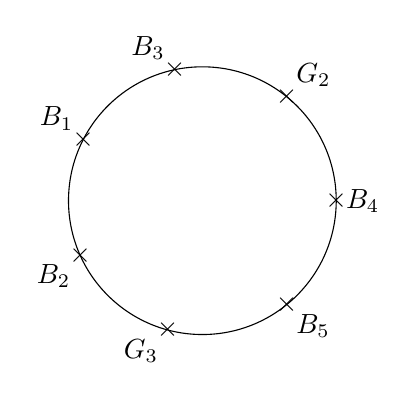
\begin{tikzpicture}
\draw (0,0) circle (1.7cm);
\draw ([shift=(51:1.7cm)]0,0) node {$\times$};
\draw ([shift=(102:1.7cm)]0,0) node {$\times$};
\draw ([shift=(153:1.7cm)]0,0) node {$\times$};
\draw ([shift=(204:1.7cm)]0,0) node {$\times$};
\draw ([shift=(255:1.7cm)]0,0) node {$\times$};
\draw ([shift=(309:1.7cm)]0,0) node {$\times$};
\draw ([shift=(0:1.7cm)]0,0) node {$\times$};
\coordinate[label=right:$B_{4}$] (C) at  ([shift=(0:1.7cm)]0,0);
\coordinate[label= above right:$G_{2}$] (C) at  ([shift=(51:1.7cm)]0,0);
\coordinate[label=above left:$B_{3}$] (C) at  ([shift=(102:1.7cm)]0,0);
\coordinate[label=above left:$B_{1}$] (C) at  ([shift=(153:1.7cm)]0,0);
\coordinate[label=below left:$B_{2}$] (C) at  ([shift=(204:1.7cm)]0,0);
\coordinate[label=below left:$G_{3}$] (C) at  ([shift=(255:1.7cm)]0,0);
\coordinate[label=below right:$B_{5}$] (C) at  ([shift=(309:1.7cm)]0,0);
\end{tikzpicture}
\caption{•}
\end{center}
\end{figure}

We may obtain another solution by using what we call the Principle of Complementation as given below: 
\begin{theorem}[Principle of Complementation (CP)  ]
If $A$ is a subset of a finite universal set $U$, then 
\[ |U\setminus A| = |U|-|A|.\]
\end{theorem}
Now, the number of ways to arrange the 5 boys and 3 girls around a table so that boy $B_1$ and girl $G_1$ are adjacent (treating $\{B_1 , G_1 \}$ as an 
entity) is 
\[(7 - 1)! \times 2 = 1440. \]
Thus the desired number of ways is by (CP), 
\[7! - 1440 = 3600.\] 
$(iii)$ We first seat the 5 boys around the table in $(5 - 1)! = 4!$ ways. 
Given such an arrangement as shown in Figure 1.3.4, there are 5 ways to 
seat girl  $G_1$ . As no girls are adjacent,  $G_2$ and  $G_3$ have 4 and 3 choices 
respectively. Thus the desired number of ways is 
\[4! \times 5 \times 4 \times 3 = 1440.\]
\end{soln}
\begin{example}
Find the number of ways to seat n married couples 
around a table in each of the following cases:\\ 
$(i)$ Men and women alternate;\\ 
$(ii)$ Every woman is next to her husband. 
\end{example}
\begin{soln}
$(i)$ The $n$ men can first be seated in $(n - 1)!$ ways. The 
$n$ women can then be seated in the $n$ spaces between two men in $n!$ ways. Thus the number of such arrangements is $(n - 1)! \times n!$.\\
$(ii)$ Each couple is first treated as an entity. The number of ways to arrange the n entities around the table is $(n -1)!$. Since the two people in each entity can be permuted in $2!$ ways, the desired number of ways is 
\[(n - 1)! \times 2^n \] 

\end{soln}
\textbf{Remark:}A famous and much more difficult problem related to the above problem is the following: How many ways are there to seat $n$ married couples $(n \ge 3)$ around a table such that men and women alternate and each woman is not adjacent to her husband? This problem, known as the problem of menages, was first introduced by the French mathematician Francis Edward Anatole Lucas (1842 - 1891). A solution to this problem will be given in Chapter 4. 

\section{Combinations}
Let $A$ be a set of $n$ distinct objects. A combination of $A$ is simply a subset of $A$. More precisely, for $0 \le r \le n$, an $r-$combination of $A$ is an $r-$element 
subset of $A$. Thus, for instance, if $A = \{a, b, c, d\}$, then the following consists of all the $3-$combinations of $A$:
\[\{ a, b, c \}, \{a, b, d\}, \{a, c, d\}, \{ b, c, d\}. \] 
There are 4 in number. Let $\comb[n]{n}$ or $\binom{n}{r}$ (which is read \say{$n$ choose $r$}) denote the 
number of $r-$combinations of an $n$-element set $A$. Then the above example says that $\comb[4]{3}=\binom{4}{3}=4$. We shall soon derive a formula for $\comb[n]{r}$.\\

What is the difference between a permutation and a combination of a set of objects? A permutation is an arrangement of certain objects and thus the ordering of objects is important, whereas a combination is just a set of objects and thus the ordering of objects is immaterial. As a matter of fact, every $r$-permutation of $A$ can be obtained in the following way: \\

$Step\,1:$ Form an $r$-combination $B$ of $A$. \\

$Step\,2:$ Arrange the $r$ objects of $B$ in a row. \\

This provides us with a means to relate the numbers P and C Indeed, 
we have by (MP): 

\end{document}